\documentclass{article}\usepackage[]{graphicx}\usepackage[]{color}
%% maxwidth is the original width if it is less than linewidth
%% otherwise use linewidth (to make sure the graphics do not exceed the margin)
\makeatletter
\def\maxwidth{ %
  \ifdim\Gin@nat@width>\linewidth
    \linewidth
  \else
    \Gin@nat@width
  \fi
}
\makeatother

\definecolor{fgcolor}{rgb}{0.345, 0.345, 0.345}
\newcommand{\hlnum}[1]{\textcolor[rgb]{0.686,0.059,0.569}{#1}}%
\newcommand{\hlstr}[1]{\textcolor[rgb]{0.192,0.494,0.8}{#1}}%
\newcommand{\hlcom}[1]{\textcolor[rgb]{0.678,0.584,0.686}{\textit{#1}}}%
\newcommand{\hlopt}[1]{\textcolor[rgb]{0,0,0}{#1}}%
\newcommand{\hlstd}[1]{\textcolor[rgb]{0.345,0.345,0.345}{#1}}%
\newcommand{\hlkwa}[1]{\textcolor[rgb]{0.161,0.373,0.58}{\textbf{#1}}}%
\newcommand{\hlkwb}[1]{\textcolor[rgb]{0.69,0.353,0.396}{#1}}%
\newcommand{\hlkwc}[1]{\textcolor[rgb]{0.333,0.667,0.333}{#1}}%
\newcommand{\hlkwd}[1]{\textcolor[rgb]{0.737,0.353,0.396}{\textbf{#1}}}%

\usepackage{framed}
\makeatletter
\newenvironment{kframe}{%
 \def\at@end@of@kframe{}%
 \ifinner\ifhmode%
  \def\at@end@of@kframe{\end{minipage}}%
  \begin{minipage}{\columnwidth}%
 \fi\fi%
 \def\FrameCommand##1{\hskip\@totalleftmargin \hskip-\fboxsep
 \colorbox{shadecolor}{##1}\hskip-\fboxsep
     % There is no \\@totalrightmargin, so:
     \hskip-\linewidth \hskip-\@totalleftmargin \hskip\columnwidth}%
 \MakeFramed {\advance\hsize-\width
   \@totalleftmargin\z@ \linewidth\hsize
   \@setminipage}}%
 {\par\unskip\endMakeFramed%
 \at@end@of@kframe}
\makeatother

\definecolor{shadecolor}{rgb}{.97, .97, .97}
\definecolor{messagecolor}{rgb}{0, 0, 0}
\definecolor{warningcolor}{rgb}{1, 0, 1}
\definecolor{errorcolor}{rgb}{1, 0, 0}
\newenvironment{knitrout}{}{} % an empty environment to be redefined in TeX

\usepackage{alltt}

\usepackage{graphicx}
\usepackage{wrapfig}
\usepackage[utf8]{inputenc}
\usepackage[english]{babel}
 
\setlength{\parindent}{2em}
\setlength{\parskip}{1em}

\graphicspath{ {images/} }


\title{Quick Tour of R and R Studio}
\date{February 12, 2106}
\author{Robert Olendorf}
\IfFileExists{upquote.sty}{\usepackage{upquote}}{}
\begin{document}
  \maketitle
  
  \pagenumbering{gobble}
  \newpage
  
  \section*{R Studio}
  

  
  R Studio is an Integrated Development Environment (IDE) for the R Statistical Package. You can run R 
  fine from the command line and using text editors such as Notepad++ or Textmate, but it provides a 
  nice comprehensive view of your current project. It's also probably easier for beginners to learn on.
  
  \begin{figure}[t]
    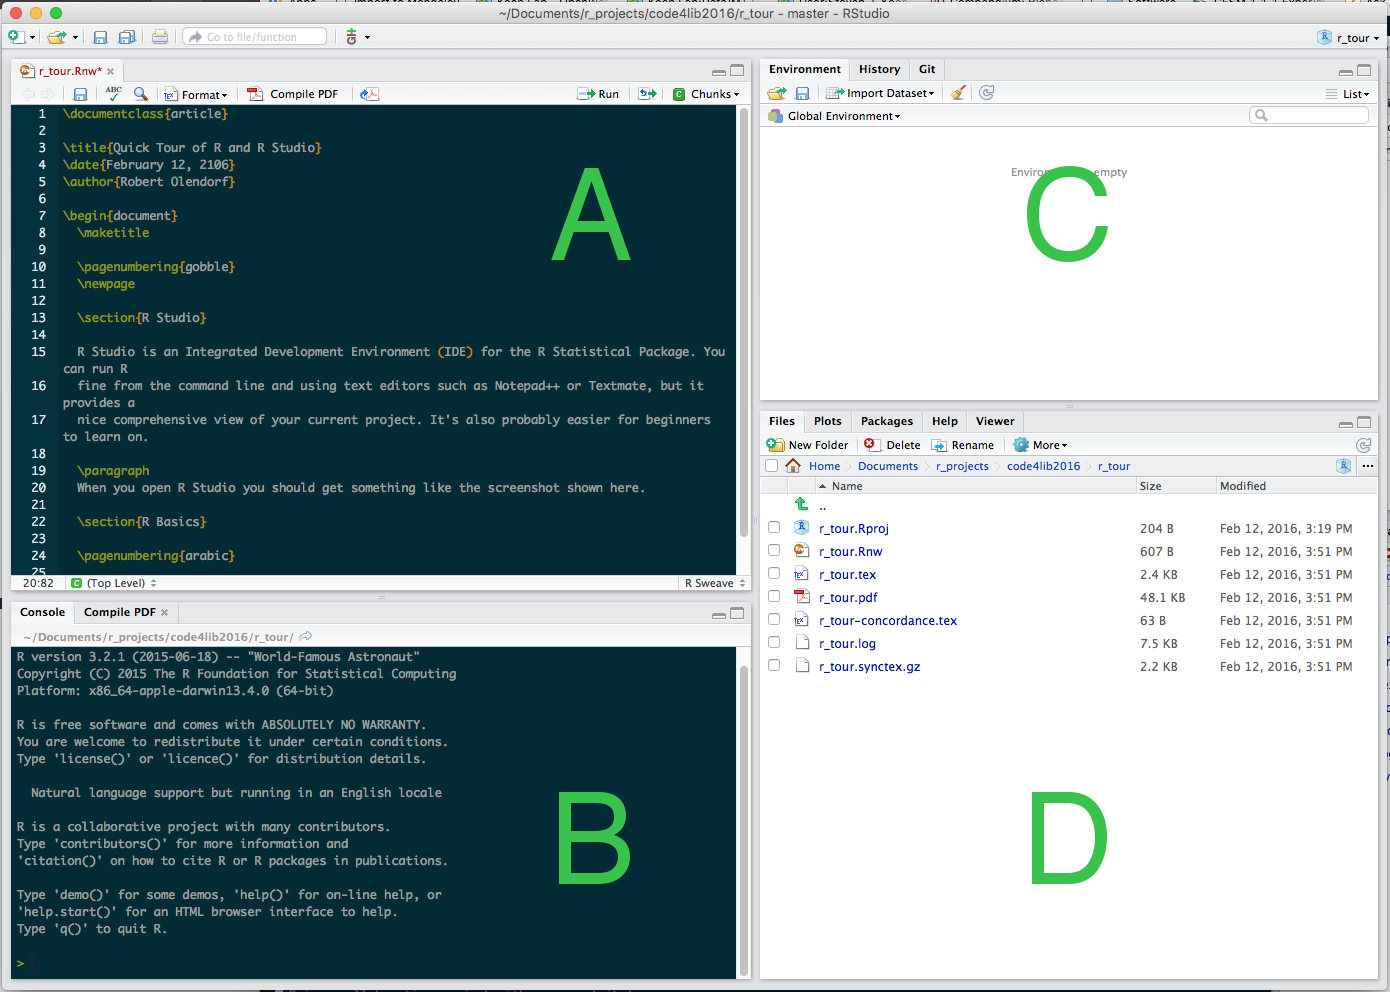
\includegraphics[scale=0.25]{rstudio_screenshot}
    \caption{Screen shot from the typical default layout.}
    \label{fig:screenshot}
    \centering
  \end{figure}
  
 When you open R Studio you should get something like the screenshot shown in figure \ref{fig:screenshot}. \textbf{Section A} is where your scripts and other documents are displayed. \textbf{Section B} is the \textbf{\textit{Console}}, where you do your interactive programming. \textbf{Section C} contains several tabs. It will usually contain at least your \textbf{\textit{Environment}}, a listing of all your objects (ie. variables, data) and a \textbf{\textit{History}} tab for your \textbf{\textit{Console}} input. \textbf{Section D} contains a number of tabs. Minimally it will contain a \textbf{\textit{Files}} tab, a \textbf{\textit{Plots}} tab, a \textbf{\textit{Packages}} tab, and a \textbf{\textit{Help}} tab. The \textbf{\textit{Files}} tab allows you to easily navigate the directory structure of your project. The \textbf{\textit{Plots}} tab displays previews of plots you generate. The \textbf{\textit{Packages}} tab lets you easily manage your R packages. The \textbf{\textit{Help}} tab displays the help.
 

\subsection*{Setting Up}
 Our first task is to define a default working direcotry. This is where R will start when you are not working on a project. Opening and saving files will be relative to this directory. Create a directory in your \textit{Documents} called \textit{rprojects}. You can of course choose your own location. Choose \textbf{[Preferences]} from the \textbf{[RStudio]} menu. Our first step will be to define a default working directory. This is where R will start, and save files if you are not working on a project. Choose \textbf{[Preferences]} the \textbf{[RStudio]} menu and choose the \textbf{[General]} tab. The top options edit or browse to set the default working directory to \textit{rprojects}.
 
 
 Next choose the \textbf{[Code]} tab. Check \textbf{Insert spaces for tab} and set it to 2. I also like to have \textbf{Insert matching parens/quotes} turned on. 
 
 Got the \textbf{[Appearance]} tab and choose an \textit{Editor Theme}. I like \textit{Solarized Dark} or \textit{Monokai} but just make sure its one that works well for you. 
 
 Unless you have a reason to change it, leave the \textbf{Pane Layout} at the defaults. It will work better with this and other tutorials.
 
 Leave the \textbf{Packages} as the default values.
 
 In the \textbf{Sweave} tab set \textit{Weave Rnw files usign: } to \textbf{\textit{Knitr}}. \textit{Typeset LaTeX into PDF using: \textbf{pdfLaTeX}}. Make sure \textit{Clean auxilliary output after compile} and \textit{Insert numbered sections and subsections} are checked. \textit{\ldots} using \textbf{\textit{RStudio Viewer}}. 
 
 Leave the \textbf{Spelling} tab at the defaults.
 
 I usually do my Git commands on a separate terminal window. However, sometimes you need to use the RStudio Git integration. To set this up in the \textbf{Git/SVN} make sure the Git executable is set up. This may vary with operating system. Also create an SSH key if you haven't already, or add the path to it if you have one.
 
 Make sure \textit{Enable publishing apps and documents} is checked in the \textbf{Publishing} tab.

 
  \section*{R Basics}
  
  \subsection*{Command Line}
    R is a command line tool. This gives many people stress, but don't let it stress you. First learn the syntax. Then learn the commands you use most often. Also, don't hesitate to Google something. I often do, especially when its something I don't do a lot. Don't waste time fiddling. 
    First off, lets do something easy. Lets do some math.
    
\begin{knitrout}
\definecolor{shadecolor}{rgb}{0.969, 0.969, 0.969}\color{fgcolor}\begin{kframe}
\begin{alltt}
\hlnum{1} \hlopt{+} \hlnum{1}  \hlcom{# R will just print the answer}
\end{alltt}
\begin{verbatim}
## [1] 2
\end{verbatim}
\begin{alltt}
\hlcom{# However, we rarely want to do this. Lets set it to a variable.}
\hlstd{a} \hlkwb{<-} \hlnum{1} \hlopt{+} \hlnum{1}  \hlcom{# a is the variable, we use the less than and dash }
            \hlcom{# rather than equals}
\hlstd{a} \hlcom{# Notice the value isn't displayed until we enter the variable}
\end{alltt}
\begin{verbatim}
## [1] 2
\end{verbatim}
\begin{alltt}
  \hlcom{# again}
\hlstd{b} \hlkwb{=} \hlnum{1} \hlopt{+} \hlnum{1} \hlcom{# Equals still works, but its not preferred. }
\end{alltt}
\end{kframe}
\end{knitrout}
    
    Variables can and function names may consist of letters, numbers, dots and underlines. They must start with a letter or a dot not followed by a number. Starting with a dot is valid, but not good style.
    
\begin{knitrout}
\definecolor{shadecolor}{rgb}{0.969, 0.969, 0.969}\color{fgcolor}\begin{kframe}
\begin{alltt}
a <- 1  \hlcom{# valid}
b.1 <- 2 \hlcom{# valid}
b1 <- 3 \hlcom{# valid}
b_1 <- 4 \hlcom{# valid }
.b <- \hlcom{# valid}
1b <- 5 \hlcom{# invalid}
.1 <- \hlcom{# invalid}
\end{alltt}
\end{kframe}
\end{knitrout}
    
    Rists tend to use the dot as a namespacing convention. However, there is no true significance to the dot in the name. R treats it as just another character.
    
    Now look in your \textbf{Environment} tab. You will see the \textbf{\textit{a}} and \textbf{\textit{b}} variables in there. Choose the \textbf{History} tab. You will see both commands recorded. Its good to get in the habit of building a script of your work. So lets do that. Do \textbf{[File/New File/R Script]}. Now select those two lines(Shift Select) and click \textbf{To Source}. It should be in your script now. This is a good way to build up scripts. Play around in the console to get it working, then copy the command(s) to a script. You may have to tweak the script still, but its an efficient way to go.
    
  \subsection*{Datatypes}
    
    Lets get some basics out of the way before we start building documents. We need to understand R Datatypes, Functions and learn some of the most basic functions first.
    
    \subsubsection*{Scalars}
    R comes with the typical scalar datatypes shown below.
    
\begin{knitrout}
\definecolor{shadecolor}{rgb}{0.969, 0.969, 0.969}\color{fgcolor}\begin{kframe}
\begin{alltt}
  \hlnum{5} \hlcom{# an integer (numeric)}
\end{alltt}
\begin{verbatim}
## [1] 5
\end{verbatim}
\begin{alltt}
  \hlnum{5.5} \hlcom{# float (numeric)}
\end{alltt}
\begin{verbatim}
## [1] 5.5
\end{verbatim}
\begin{alltt}
  \hlstr{"a"} \hlcom{#character}
\end{alltt}
\begin{verbatim}
## [1] "a"
\end{verbatim}
\begin{alltt}
  \hlstr{"a string"}  \hlcom{# a string (a vector of characters)}
\end{alltt}
\begin{verbatim}
## [1] "a string"
\end{verbatim}
\begin{alltt}
  \hlnum{FALSE} \hlcom{# logical}
\end{alltt}
\begin{verbatim}
## [1] FALSE
\end{verbatim}
\end{kframe}
\end{knitrout}
    
    \subsubsection*{Vectors}
\begin{knitrout}
\definecolor{shadecolor}{rgb}{0.969, 0.969, 0.969}\color{fgcolor}\begin{kframe}
\begin{alltt}
  \hlstd{num.vec} \hlkwb{<-} \hlkwd{c}\hlstd{(}\hlnum{1}\hlstd{,} \hlnum{2}\hlstd{,} \hlnum{4}\hlstd{,} \hlnum{5}\hlstd{)}  \hlcom{# creating a vector the hard way}
  \hlstd{num.vec}
\end{alltt}
\begin{verbatim}
## [1] 1 2 4 5
\end{verbatim}
\begin{alltt}
  \hlstd{num.vec2} \hlkwb{<-} \hlnum{1}\hlopt{:}\hlnum{5} \hlcom{# automating a vector creation}
  \hlstd{num.vec2}
\end{alltt}
\begin{verbatim}
## [1] 1 2 3 4 5
\end{verbatim}
\begin{alltt}
  \hlstd{num.vec3} \hlkwb{<-} \hlkwd{seq}\hlstd{(}\hlnum{1}\hlstd{,} \hlnum{5}\hlstd{,} \hlnum{0.5}\hlstd{)}
  \hlstd{num.vec3}
\end{alltt}
\begin{verbatim}
## [1] 1.0 1.5 2.0 2.5 3.0 3.5 4.0 4.5 5.0
\end{verbatim}
\begin{alltt}
  \hlstd{alpha.vec} \hlkwb{<-} \hlkwd{c}\hlstd{(}\hlstr{"a"}\hlstd{,} \hlstr{"b"}\hlstd{,} \hlstr{"c"}\hlstd{,} \hlstr{"d"}\hlstd{)}  \hlcom{# a vector of charaters}
  \hlstd{alpha.vec}
\end{alltt}
\begin{verbatim}
## [1] "a" "b" "c" "d"
\end{verbatim}
\begin{alltt}
  \hlcom{# a vector of logicals}
  \hlstd{logical.vec} \hlkwb{<-} \hlkwd{c}\hlstd{(}\hlnum{TRUE}\hlstd{,} \hlnum{FALSE}\hlstd{,} \hlnum{TRUE}\hlstd{,} \hlnum{TRUE}\hlstd{,} \hlnum{FALSE}\hlstd{)}
  \hlstd{logical.vec}
\end{alltt}
\begin{verbatim}
## [1]  TRUE FALSE  TRUE  TRUE FALSE
\end{verbatim}
\begin{alltt}
  \hlcom{##}
  \hlcom{# A vector must be of the same type. }
   \hlcom{# The integer gets converted to a character}
  \hlstd{test.vec} \hlkwb{<-} \hlkwd{c}\hlstd{(}\hlstr{"1"}\hlstd{,} \hlstr{"2"}\hlstd{,} \hlnum{3}\hlstd{)}
  \hlstd{test.vec}
\end{alltt}
\begin{verbatim}
## [1] "1" "2" "3"
\end{verbatim}
\end{kframe}
\end{knitrout}
    
    You can access parts of vectors using the following methods.
    
\begin{knitrout}
\definecolor{shadecolor}{rgb}{0.969, 0.969, 0.969}\color{fgcolor}\begin{kframe}
\begin{alltt}
  \hlstd{v} \hlkwb{<-} \hlkwd{seq}\hlstd{(}\hlnum{1}\hlstd{,} \hlnum{20}\hlstd{,} \hlnum{2}\hlstd{)}
  \hlstd{v}
\end{alltt}
\begin{verbatim}
##  [1]  1  3  5  7  9 11 13 15 17 19
\end{verbatim}
\begin{alltt}
  \hlcom{# Get 1 item. Notice the index starts with 1 rather than}
  \hlcom{# 0 as in other languages.}
  \hlstd{v[}\hlnum{1}\hlstd{]}
\end{alltt}
\begin{verbatim}
## [1] 1
\end{verbatim}
\begin{alltt}
  \hlstd{v[}\hlnum{2}\hlopt{:}\hlnum{5}\hlstd{]}  \hlcom{# Get a slice}
\end{alltt}
\begin{verbatim}
## [1] 3 5 7 9
\end{verbatim}
\begin{alltt}
  \hlstd{v[}\hlkwd{c}\hlstd{(}\hlnum{1}\hlstd{,} \hlnum{5}\hlstd{,} \hlnum{9}\hlstd{)]}  \hlcom{# Get specific indices}
\end{alltt}
\begin{verbatim}
## [1]  1  9 17
\end{verbatim}
\end{kframe}
\end{knitrout}
    
    \subsubsection*{Matrixes}
    Matrices are two dimensional vectors. Columns (but not row) in a matrix must have the same datatype (numeric, character, etc.).
    
\begin{knitrout}
\definecolor{shadecolor}{rgb}{0.969, 0.969, 0.969}\color{fgcolor}\begin{kframe}
\begin{alltt}
  \hlcom{# Create a 5 x 4 matrix. R fills by column.}
  \hlstd{matrix.1} \hlkwb{<-} \hlkwd{matrix}\hlstd{(}\hlnum{1}\hlopt{:}\hlnum{20}\hlstd{,} \hlkwc{nrow}\hlstd{=}\hlnum{5}\hlstd{,} \hlkwc{ncol}\hlstd{=}\hlnum{4}\hlstd{)}
  \hlstd{matrix.1}
\end{alltt}
\begin{verbatim}
##      [,1] [,2] [,3] [,4]
## [1,]    1    6   11   16
## [2,]    2    7   12   17
## [3,]    3    8   13   18
## [4,]    4    9   14   19
## [5,]    5   10   15   20
\end{verbatim}
\begin{alltt}
  \hlcom{# You can fill by rows too}

  \hlstd{matrix.row} \hlkwb{<-} \hlkwd{matrix}\hlstd{(}\hlnum{1}\hlopt{:}\hlnum{20}\hlstd{,} \hlkwc{nrow} \hlstd{=} \hlnum{5}\hlstd{,} \hlkwc{ncol}\hlstd{=}\hlnum{4}\hlstd{,} \hlkwc{byrow} \hlstd{=} \hlnum{TRUE}\hlstd{)}
  \hlstd{matrix.row}
\end{alltt}
\begin{verbatim}
##      [,1] [,2] [,3] [,4]
## [1,]    1    2    3    4
## [2,]    5    6    7    8
## [3,]    9   10   11   12
## [4,]   13   14   15   16
## [5,]   17   18   19   20
\end{verbatim}
\begin{alltt}
  \hlcom{# If you don't fill the matrix R repeats}
  \hlcom{# the sequence until its filled. It doesn't}
  \hlcom{# have to be an even fill, but you will get a warning.}
  \hlstd{matrix.2} \hlkwb{<-} \hlkwd{matrix}\hlstd{(}\hlnum{1}\hlopt{:}\hlnum{7}\hlstd{,} \hlkwc{nrow}\hlstd{=}\hlnum{5}\hlstd{,} \hlkwc{ncol}\hlstd{=}\hlnum{4}\hlstd{)}
\end{alltt}


{\ttfamily\noindent\color{warningcolor}{\#\# Warning in matrix(1:7, nrow = 5, ncol = 4): data length [7] is not a sub-multiple or multiple of the number of rows [5]}}\begin{alltt}
  \hlstd{matrix.2}
\end{alltt}
\begin{verbatim}
##      [,1] [,2] [,3] [,4]
## [1,]    1    6    4    2
## [2,]    2    7    5    3
## [3,]    3    1    6    4
## [4,]    4    2    7    5
## [5,]    5    3    1    6
\end{verbatim}
\end{kframe}
\end{knitrout}
    
    Accessing a matrix is as follows.
    
\begin{knitrout}
\definecolor{shadecolor}{rgb}{0.969, 0.969, 0.969}\color{fgcolor}\begin{kframe}
\begin{alltt}
  \hlstd{matrix.1[,}\hlnum{3}\hlstd{]}  \hlcom{# 4th column}
\end{alltt}
\begin{verbatim}
## [1] 11 12 13 14 15
\end{verbatim}
\begin{alltt}
  \hlstd{matrix.1[}\hlnum{2}\hlstd{,]}  \hlcom{# 2nd row}
\end{alltt}
\begin{verbatim}
## [1]  2  7 12 17
\end{verbatim}
\begin{alltt}
  \hlstd{matrix.1[}\hlnum{2}\hlopt{:}\hlnum{4}\hlstd{,} \hlnum{1}\hlopt{:}\hlnum{3}\hlstd{]} \hlcom{# rows 2, 3 ,4 of columuns 1, 2, 3}
\end{alltt}
\begin{verbatim}
##      [,1] [,2] [,3]
## [1,]    2    7   12
## [2,]    3    8   13
## [3,]    4    9   14
\end{verbatim}
\end{kframe}
\end{knitrout}
    
    \subsubsection*{Lists}
    
    Lists are an ordered collection of objects. They don't have to be the same type.
    
\begin{knitrout}
\definecolor{shadecolor}{rgb}{0.969, 0.969, 0.969}\color{fgcolor}\begin{kframe}
\begin{alltt}
  \hlcom{# A list with a string, numeric, logical and a vector}
  \hlcom{# using a variable to insert the vector.}
  \hlstd{list.1} \hlkwb{<-} \hlkwd{list}\hlstd{(}\hlstr{"Fred"}\hlstd{,} \hlnum{24}\hlstd{,} \hlnum{FALSE}\hlstd{, num.vec)}
  \hlstd{list.1}
\end{alltt}
\begin{verbatim}
## [[1]]
## [1] "Fred"
## 
## [[2]]
## [1] 24
## 
## [[3]]
## [1] FALSE
## 
## [[4]]
## [1] 1 2 4 5
\end{verbatim}
\begin{alltt}
  \hlcom{# Named list components}
  \hlstd{list.2} \hlkwb{<-} \hlkwd{list}\hlstd{(}\hlkwc{name}\hlstd{=}\hlstr{"Sue"}\hlstd{,} \hlkwc{age}\hlstd{=}\hlnum{32}\hlstd{,} \hlkwc{smoker}\hlstd{=}\hlnum{TRUE}\hlstd{,} \hlkwc{data}\hlstd{=num.vec2)}
  \hlstd{list.2}
\end{alltt}
\begin{verbatim}
## $name
## [1] "Sue"
## 
## $age
## [1] 32
## 
## $smoker
## [1] TRUE
## 
## $data
## [1] 1 2 3 4 5
\end{verbatim}
\begin{alltt}
  \hlcom{# We can make a vector of lists}

  \hlstd{list.vect} \hlkwb{<-} \hlkwd{c}\hlstd{(list.1, list.2)}
  \hlstd{list.vect}
\end{alltt}
\begin{verbatim}
## [[1]]
## [1] "Fred"
## 
## [[2]]
## [1] 24
## 
## [[3]]
## [1] FALSE
## 
## [[4]]
## [1] 1 2 4 5
## 
## $name
## [1] "Sue"
## 
## $age
## [1] 32
## 
## $smoker
## [1] TRUE
## 
## $data
## [1] 1 2 3 4 5
\end{verbatim}
\end{kframe}
\end{knitrout}
    
    We can access parts of a list like this.
    
\begin{knitrout}
\definecolor{shadecolor}{rgb}{0.969, 0.969, 0.969}\color{fgcolor}\begin{kframe}
\begin{alltt}
  \hlcom{# Notice the double bracket.}
  \hlstd{list.2[[}\hlnum{2}\hlstd{]]}  \hlcom{# the second entry}
\end{alltt}
\begin{verbatim}
## [1] 32
\end{verbatim}
\begin{alltt}
  \hlstd{list.2[[}\hlstr{"name"}\hlstd{]]}
\end{alltt}
\begin{verbatim}
## [1] "Sue"
\end{verbatim}
\end{kframe}
\end{knitrout}
    
    \subsubsection*{Data Frames}
    Data frames are something fairly unique to R. It is usually what  you will
    use to contain tabuluar data. They are a bit like matrices, but each column 
    can have a different datatype. 
    
\begin{knitrout}
\definecolor{shadecolor}{rgb}{0.969, 0.969, 0.969}\color{fgcolor}\begin{kframe}
\begin{alltt}
  \hlstd{a} \hlkwb{<-} \hlkwd{c}\hlstd{(}\hlnum{1}\hlopt{:}\hlnum{4}\hlstd{)}
  \hlstd{b} \hlkwb{<-} \hlkwd{c}\hlstd{(}\hlstr{"George"}\hlstd{,} \hlstr{"Tom"}\hlstd{,} \hlstr{"Phineas"}\hlstd{,} \hlstr{"Ferb"}\hlstd{)}
  \hlstd{c} \hlkwb{<-} \hlkwd{c}\hlstd{(}\hlnum{TRUE}\hlstd{,} \hlnum{FALSE}\hlstd{,} \hlnum{FALSE}\hlstd{,} \hlnum{TRUE}\hlstd{)}

  \hlstd{df.1} \hlkwb{<-} \hlkwd{data.frame}\hlstd{(a, b, c)}
  \hlstd{df.1}
\end{alltt}
\begin{verbatim}
##   a       b     c
## 1 1  George  TRUE
## 2 2     Tom FALSE
## 3 3 Phineas FALSE
## 4 4    Ferb  TRUE
\end{verbatim}
\begin{alltt}
  \hlcom{# We can name the columsn as well.}
  \hlkwd{names}\hlstd{(df.1)} \hlkwb{<-} \hlkwd{c}\hlstd{(}\hlstr{"ID"}\hlstd{,} \hlstr{"name"}\hlstd{,} \hlstr{"smoker"}\hlstd{)}
  \hlstd{df.1}
\end{alltt}
\begin{verbatim}
##   ID    name smoker
## 1  1  George   TRUE
## 2  2     Tom  FALSE
## 3  3 Phineas  FALSE
## 4  4    Ferb   TRUE
\end{verbatim}
\end{kframe}
\end{knitrout}
    
    We can access parts of a data frame
    
\begin{knitrout}
\definecolor{shadecolor}{rgb}{0.969, 0.969, 0.969}\color{fgcolor}\begin{kframe}
\begin{alltt}
  \hlstd{df.1[}\hlnum{2}\hlopt{:}\hlnum{4}\hlstd{]}  \hlcom{# columuns 2 - 4}
\end{alltt}


{\ttfamily\noindent\bfseries\color{errorcolor}{\#\# Error in `[.data.frame`(df.1, 2:4): undefined columns selected}}\begin{alltt}
  \hlstd{df.1[}\hlkwd{c}\hlstd{(}\hlstr{"ID"}\hlstd{,} \hlstr{"name"}\hlstd{)]}  \hlcom{# columns by name}
\end{alltt}
\begin{verbatim}
##   ID    name
## 1  1  George
## 2  2     Tom
## 3  3 Phineas
## 4  4    Ferb
\end{verbatim}
\begin{alltt}
  \hlstd{df.1}\hlopt{$}\hlstd{ID}  \hlcom{# variable ID (or column ID)}
\end{alltt}
\begin{verbatim}
## [1] 1 2 3 4
\end{verbatim}
\end{kframe}
\end{knitrout}
    
    \subsubsection*{Factors}
    
    Sometimes our variable is categorical (nominal). WE can tell R this by 
    creating a factor.
    
\begin{knitrout}
\definecolor{shadecolor}{rgb}{0.969, 0.969, 0.969}\color{fgcolor}\begin{kframe}
\begin{alltt}
  \hlstd{color} \hlkwb{<-} \hlkwd{c}\hlstd{(}\hlkwd{rep}\hlstd{(}\hlstr{"red"}\hlstd{,} \hlnum{21}\hlstd{),} \hlkwd{rep}\hlstd{(}\hlstr{"green"}\hlstd{,} \hlnum{14}\hlstd{),} \hlkwd{rep}\hlstd{(}\hlstr{"blue"}\hlstd{,} \hlnum{18}\hlstd{))}
  \hlkwd{head}\hlstd{(color)}
\end{alltt}
\begin{verbatim}
## [1] "red" "red" "red" "red" "red" "red"
\end{verbatim}
\begin{alltt}
  \hlstd{color.factor} \hlkwb{<-} \hlkwd{factor}\hlstd{(color)}
  \hlkwd{head}\hlstd{(color.factor)}
\end{alltt}
\begin{verbatim}
## [1] red red red red red red
## Levels: blue green red
\end{verbatim}
\begin{alltt}
  \hlcom{# Summary will work on color.factor but not color}
  \hlkwd{summary}\hlstd{(color)}
\end{alltt}
\begin{verbatim}
##    Length     Class      Mode 
##        53 character character
\end{verbatim}
\begin{alltt}
  \hlkwd{summary}\hlstd{(color.factor)}
\end{alltt}
\begin{verbatim}
##  blue green   red 
##    18    14    21
\end{verbatim}
\end{kframe}
\end{knitrout}
    
    
  \subsection*{Functions}
  Functions in R look like \textbf{\textit{mean()}}. You've already seen some 
  of them being used. We use them like this.
  
\begin{knitrout}
\definecolor{shadecolor}{rgb}{0.969, 0.969, 0.969}\color{fgcolor}\begin{kframe}
\begin{alltt}
    \hlkwd{mean}\hlstd{(}\hlnum{1}\hlopt{:}\hlnum{10}\hlstd{)} \hlcom{# Gets the mean of the vector of values}
\end{alltt}
\begin{verbatim}
## [1] 5.5
\end{verbatim}
\begin{alltt}
    \hlkwd{mean}\hlstd{()} \hlcom{# Will throw a "useful" error message}
\end{alltt}


{\ttfamily\noindent\bfseries\color{errorcolor}{\#\# Error in mean.default(): argument "{}x"{} is missing, with no default}}\begin{alltt}
    \hlstd{mean} \hlcom{# will show the source code or somethign similar}
\end{alltt}
\begin{verbatim}
## function (x, ...) 
## UseMethod("mean")
## <bytecode: 0x7fb7cd88b748>
## <environment: namespace:base>
\end{verbatim}
\end{kframe}
\end{knitrout}
  
  \subsubsection*{Useful Functions}
    \begin{description}
      \item[getwd()] \hfill \\
      Gets the current working directory.
      \item[setwd()] \hfill \\
      Sets teh current working directory.
      \item[help()] \hfill \\
      Gets help for something (eg help("mean"))
      \item[data()] \hfill \\
      Lists currently installed demo data sets.
    \end{description}
  
  \subsection*{A Quick Analysis}
  
  Just as an example we can do a simple analysis. We are going to use the built in \textit{cars} dataset. First click the \textbf{\textit{broom}} icon in your \textbf{\textit{Environment}} tab. For a real analysis we would also be saving useful code to an R Script or similar document, but we'll skip that for now.
  
  First we'll load the data set and get to know the data a little.
  
  
\begin{knitrout}
\definecolor{shadecolor}{rgb}{0.969, 0.969, 0.969}\color{fgcolor}\begin{kframe}
\begin{alltt}
  \hlkwd{data}\hlstd{(}\hlstr{"cars"}\hlstd{)}  \hlcom{# load the data }

  \hlcom{# "Peak at the data to see what it looks like}
  \hlkwd{head}\hlstd{(cars)}
\end{alltt}
\begin{verbatim}
##   speed dist
## 1     4    2
## 2     4   10
## 3     7    4
## 4     7   22
## 5     8   16
## 6     9   10
\end{verbatim}
\begin{alltt}
  \hlkwd{help}\hlstd{(cars)}  \hlcom{# Look at the help.}
\end{alltt}
\end{kframe}
\end{knitrout}
  
   We see that the \textit{cars} data set is just two columun, speed and distance. First lets get look at the data itself before we analyze it.
  
\begin{knitrout}
\definecolor{shadecolor}{rgb}{0.969, 0.969, 0.969}\color{fgcolor}\begin{kframe}
\begin{alltt}
    \hlkwd{summary}\hlstd{(cars)} \hlcom{# Simple descriptive statistics}
\end{alltt}
\begin{verbatim}
##      speed           dist       
##  Min.   : 4.0   Min.   :  2.00  
##  1st Qu.:12.0   1st Qu.: 26.00  
##  Median :15.0   Median : 36.00  
##  Mean   :15.4   Mean   : 42.98  
##  3rd Qu.:19.0   3rd Qu.: 56.00  
##  Max.   :25.0   Max.   :120.00
\end{verbatim}
\end{kframe}
\end{knitrout}
  
\begin{knitrout}
\definecolor{shadecolor}{rgb}{0.969, 0.969, 0.969}\color{fgcolor}\begin{kframe}
\begin{alltt}
    \hlcom{# Boxplots are good to see the distribution}
    \hlcom{# and detecting outliers. This looks good.}
    \hlkwd{boxplot}\hlstd{(cars,} \hlkwc{notch}\hlstd{=}\hlnum{TRUE}\hlstd{)}
\end{alltt}
\end{kframe}
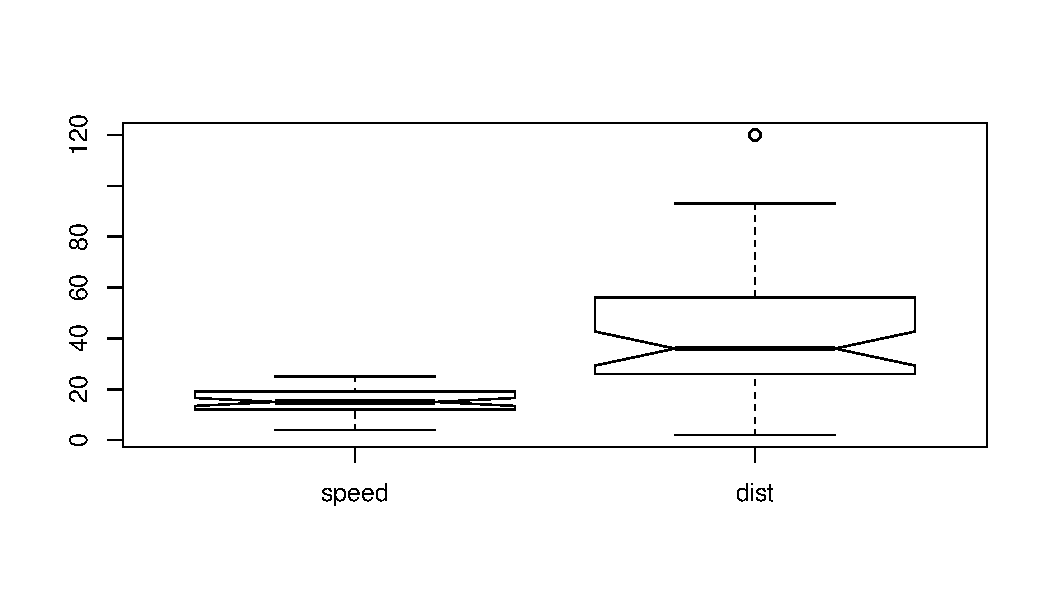
\includegraphics[width=\maxwidth]{figure/cars-boxplot-1} 

\end{knitrout}
  
\begin{knitrout}
\definecolor{shadecolor}{rgb}{0.969, 0.969, 0.969}\color{fgcolor}\begin{kframe}
\begin{alltt}
    \hlcom{# We can also do histograms.}
    \hlkwd{hist}\hlstd{(cars}\hlopt{$}\hlstd{speed)}
\end{alltt}
\end{kframe}
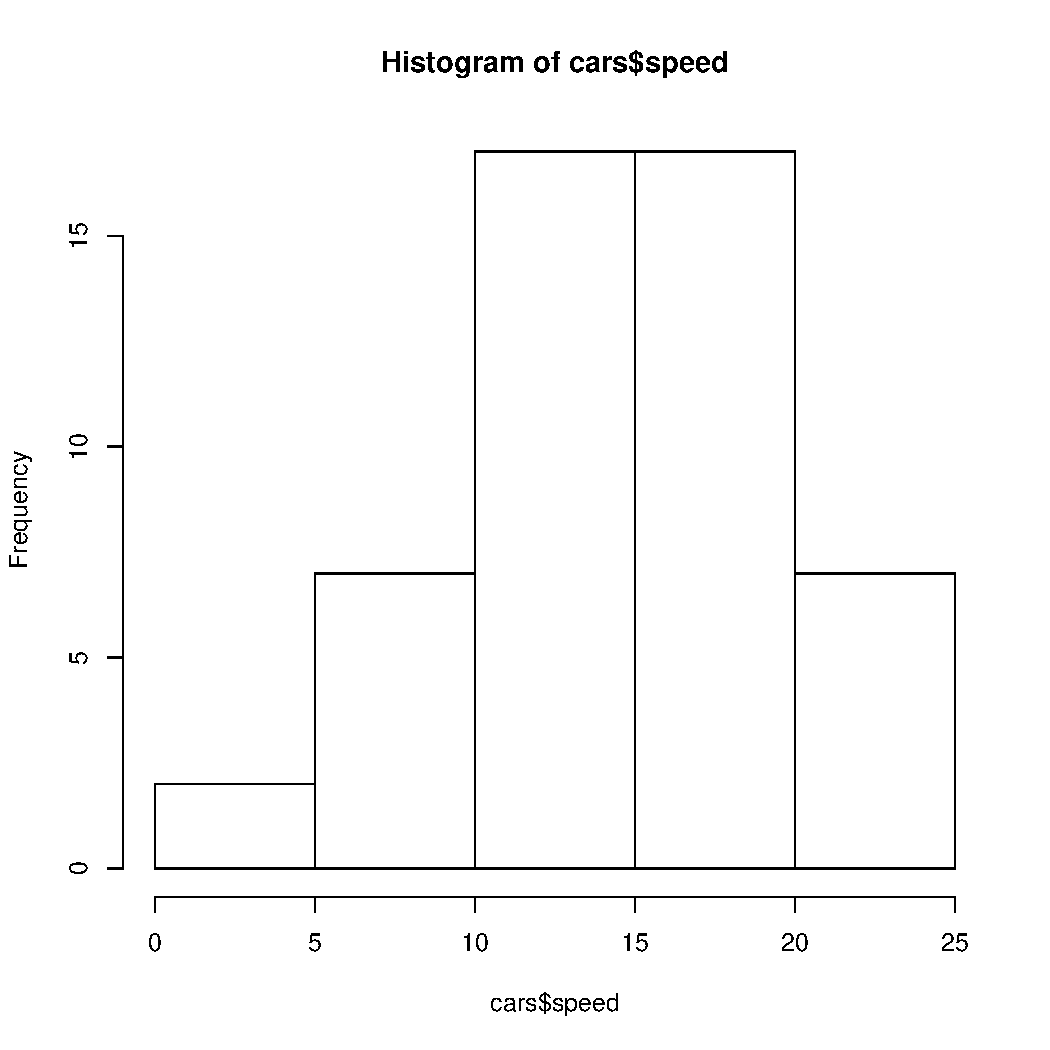
\includegraphics[width=\maxwidth]{figure/cars-histogram1-1} 

\end{knitrout}
\begin{knitrout}
\definecolor{shadecolor}{rgb}{0.969, 0.969, 0.969}\color{fgcolor}\begin{kframe}
\begin{alltt}
    \hlkwd{hist}\hlstd{(cars}\hlopt{$}\hlstd{dist)}
\end{alltt}
\end{kframe}
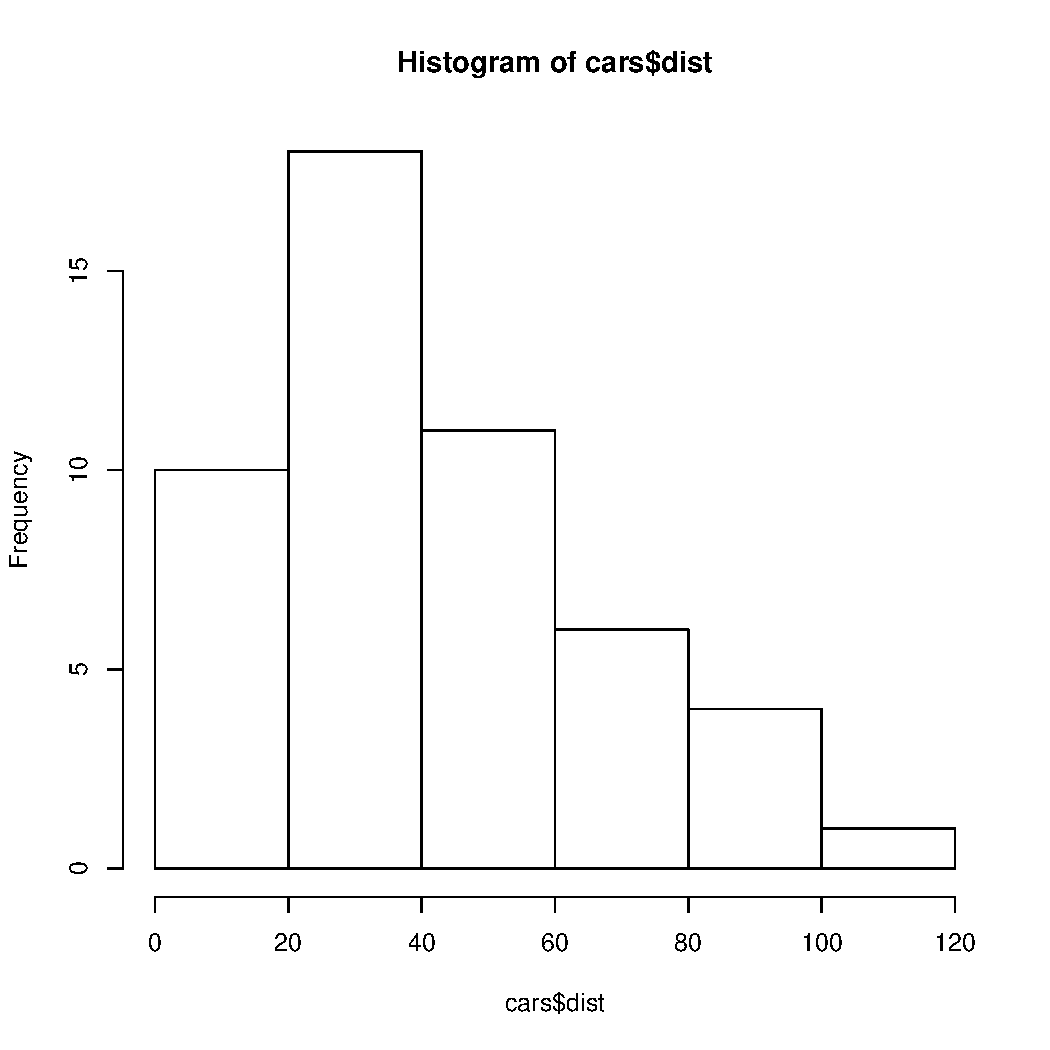
\includegraphics[width=\maxwidth]{figure/cars-histogram2-1} 

\end{knitrout}
  
  
  \pagenumbering{arabic}


\end{document}
